\section{Spread impact in price response functions}\label{sec:spread_impact}


As we showed in Sect. \ref{sec:introduction}, due to the difference in the position of the decimal
points between foreign exchange rates, we need to introduce a ``scaling factor''
with the purpose of bringing the pip to the left of the decimal point.
For example, the scaling factor for the USD/JPY is $100$ and that for the
EUR/USD is $10000$.

The pip bid-ask spread is defined as \cite{micro_eff}:

\begin{equation}
    \text{pip}_{spread} = \left(a\left(t\right) - b\left(t\right)\right) \cdot \text{scaling factor}
\end{equation}

\begin{figure*}[htbp]
    \centering
    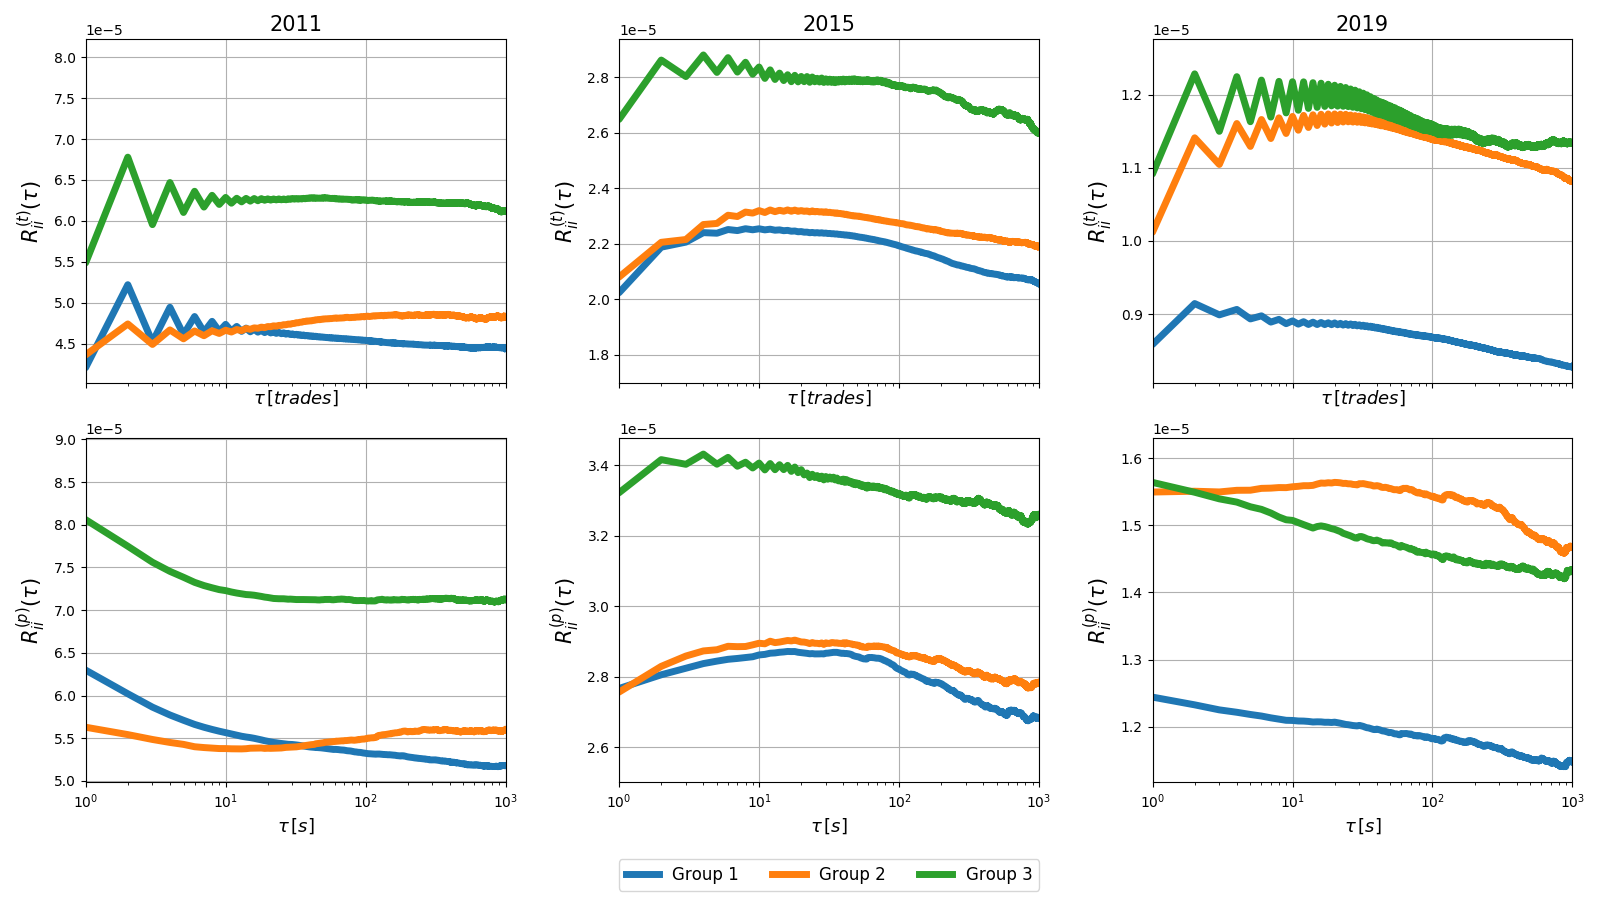
\includegraphics[width=\textwidth]{figures/05_spread_impact.png}
    \caption{Average price response functions
             $R^{\left(t\right)}_{ii}\left(\tau\right)$ versus time lag $\tau$
             on a logarithmic scale in trade time scale (Top) and
             $R^{\left(p\right)}_{ii}\left(\tau\right)$ excluding
             $\varepsilon^{\left(p\right)}_{i}\left(t\right) = 0$ versus time
             lag $\tau$ on a logarithmic scale in physical time scale (Bottom)
             for 47 foreign exchange pairs divided in three representative
             groups in three different years (2011, 2015 and 2019).}
    \label{fig:spread_impact}
\end{figure*}